\scanpage{26}
\mspage{13}
considérer que \deleted{\unsure{le|que}} $\unsure{\tau|\mathcal T}$
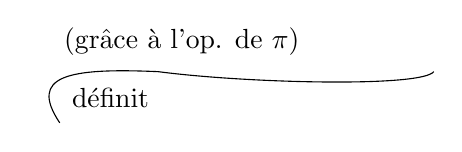
\begin{tikzpicture}[baseline=(main.base),x=1cm,y=1cm]
\node[anchor=base west,inner sep=0pt] (main) at (0,0) {définit};
\node[anchor=south west,inner sep=0pt] at (-0.10,0.65) {\inserted{(grâce à l'op. de $\pi$)}};
\draw[thin] (-0.15,-0.20) .. controls (-0.55,0.40) and (-0.05,0.50) .. (1.10,0.45) .. controls (2.25,0.30) and (4.45,0.25) .. (4.60,0.45);
\end{tikzpicture}
un foncteur
\diagram{\begin{tikzcd}[ampersand replacement=\&,row sep=large,column sep=huge]
\operatorname{Rev}(\Pi)\arrow[r,"F"]\&(\operatorname{Ens})\\
(\pi\text{-}\operatorname{Ens})\arrow[u,"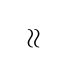
\begin{tikzpicture}[baseline=-.4ex]\node[rotate=90,inner sep=0pt] {$\approx$};\end{tikzpicture}"',"\begin{gathered}\deleted{\text{via : }\widetilde\Pi}\\E\longmapsto\widetilde\Pi^{\circ}\times_\pi E\end{gathered}"]\arrow[ur,bend right=25,"E\longmapsto\unsure{\tau|\mathcal T}^{\circ}\mathbin{\wedge}_{\pi}E"']
\end{tikzcd}}
[\uline{NB} l'indice $\circ$ indique qu'on a renversé les op. de $\pi$, pour faire opérer $\pi$ à dr)
foncteur commutant aux $\varinjlim$ quelconques. Ceci dit, on veut que $\unsure{\Gamma|F}$ (qui opère sur $\operatorname{Rev}(\Pi)$ via ses opérations sur $\Pi$) soit compatible avec le foncteur $F$, i.e. qu'on ait des isom
\[
F({}^{\gamma}\Pi')\simeq F(\Pi')
\]
$(\Pi'\in\operatorname{Ob}\operatorname{Rev}\Pi)$ fonctoriels en $\Pi'$, et avec transitivité pour $\gamma$ variable. On trouve que cela signifie
\mspage{25}
